\documentclass{article}

% ---------------------------------------------------------------------------------------------------------------
% Follow-up to "When Does a Small Sensor-Only Model Beat Time-Series Foundation Models? A Pre-Registered Evaluation
% on Indian Air Quality". Build: pdflatex main && bibtex main && pdflatex main && pdflatex main
% Every number is copied from a Kaggle log or results file named in the text; rules are in atlas/README.md
% ("ICML programme" and "Atlas v1.4 programme"), committed before the runs they govern.
% ---------------------------------------------------------------------------------------------------------------
\newif\ifpreprint
\preprinttrue
\ifpreprint
  \usepackage[preprint]{neurips_2025}
\else
  \usepackage{neurips_2025}
\fi
\makeatletter
\renewcommand{\@neuripsordinal}{41st}
\renewcommand{\@neuripsyear}{2027}
\makeatother

\usepackage[utf8]{inputenc}
\usepackage{hyperref}
\usepackage{float}
\usepackage{url}
\usepackage{booktabs}
\usepackage{amsfonts,amsmath}
\usepackage{microtype}
\usepackage{xcolor}
\usepackage{graphicx}
\usepackage{tabularx}
\usepackage{caption}
\captionsetup{font=small,labelfont=bf}
\usepackage{enumitem}
\usepackage{tikz}
\usetikzlibrary{positioning,arrows.meta,fit,calc,backgrounds,patterns}
\setlist{leftmargin=1.3em,itemsep=1pt,topsep=2pt}

\definecolor{atlasblue}{HTML}{1F5FBF}
\hypersetup{colorlinks=true,linkcolor=atlasblue!75!black,citecolor=atlasblue!75!black,urlcolor=atlasblue!75!black}
\newcommand{\pmu}{\ensuremath{\mu\mathrm{g/m^3}}}
\newcommand{\pmtf}{PM$_{2.5}$}
\newcommand{\trk}[1]{\textsc{#1}}
% I1 numbers (filled from Kaggle run atlas-i1-score)
\newcommand{\IoneRMSE}{\textbf{54.24}}\newcommand{\IoneMAE}{\textbf{31.27}}\newcommand{\IoneMBE}{$-8.66$}\newcommand{\IoneR}{\textbf{0.85}}
\newcommand{\IoneMAPE}{\textbf{21}}\newcommand{\IoneObs}{159}\newcommand{\IoneHours}{3{,}624}

\title{Atlas-F: A Small Indian Sensor Model Fused with a Foundation Model, Confirmed Across India and Set Against India's Operational Air-Quality Forecasts}

\ifpreprint
\author{%
  Aditya Kumar \qquad Anupam Singh\\
  ParadoxAI Lab\\
  \texttt{contact.paradoxailab@gmail.com}
}
\else
\author{Anonymous Author(s)\\Affiliation\\Address\\\texttt{email}}
\fi

\begin{document}
\maketitle

\begin{abstract}
A sub-million-parameter model trained only on Indian monitoring-station data, Atlas, was reported to beat
time-series foundation models at forecasting \pmtf{} 24 hours ahead. We continue that work under the same
pre-registered protocol. A confirmation test that repeats its recipe with each of four networks left out of
pre-training succeeds in Uttar Pradesh but fails in Maharashtra and Karnataka, where the station graph harms stations
the model never trained on. We repair this with Atlas-F, which averages Atlas with TimesFM~2.5 using weights re-chosen
every day from the previous 30 days only. On the all-India test (14 networks, 263 stations) Atlas-F beats Atlas
($-1.2\%$ / $-2.0\%$) and TimesFM~2.5 ($-7.2\%$ / $-6.8\%$) on trained and never-trained stations ($p<10^{-13}$), and
has lower error than TimesFM~2.5 in all 28 network-tracks, meeting a dominance rule fixed before the run. Against
India's operational forecasts, which publish no archive, we score an Atlas trained on nothing after 30 September 2024 on
the quantity an independent evaluation used for IITM's WRF-Chem and IMD's SILAM: Delhi's average hourly \pmtf{} in
winter 2024--25. Atlas's error (RMSE 54.2, MAE 31.3\,\pmu{}) is below the published Day-1 errors of WRF-Chem (92.5, 58.8) and SILAM (108.0, 71.7), as predicted before the run; the comparison is by number only, and a same-hour-yesterday forecast is also below both, which we discuss. We report every failure, including a discarded scoring run.
\end{abstract}

% =================================================================================================================
\section{Introduction}
\label{sec:intro}

Time-series foundation models (TSFMs) forecast new series zero-shot~\citep{das2024timesfm,ansari2024chronos,woo2024moirai}.
Our first paper~\citep{atlas1} showed that Atlas, a 0.97M-parameter model trained only on Indian station data, beats
them on Indian \pmtf{}: across India by 6.1\% and 4.8\% on trained and never-trained stations, and on Delhi against six
TSFMs. Two questions were left open. The Delhi result rested on a test period scored by several versions, so it needed
confirmation on networks no version had been tuned on. And Atlas had not been set against the forecasts India actually
issues, IITM's Air Quality Early Warning System~\citep{jena2021delhi400m} and IMD's SILAM, because neither publishes an
archive of past forecasts.

This paper answers both, under the protocol of~\citep{atlas1}: every rule and most predictions were committed to a
public repository before the runs they govern, every comparison is a Diebold--Mariano test on trained and
never-trained stations separately, and failures are reported with the same weight as successes. Our contributions:
\begin{itemize}
\item \textbf{A confirmation test that partly failed} (\S\ref{sec:lono}). With each of four networks left out of
  pre-training, the recipe beats TimesFM~2.5 in Uttar Pradesh, is level in Haryana and loses in Maharashtra and
  Karnataka. The losses locate a specific failure: the station graph misleads never-trained stations where cities are
  far apart.
\item \textbf{Atlas-F} (\S\ref{sec:arch}, \S\ref{sec:fusion}), a fused system whose weights between Atlas and
  TimesFM~2.5 are learned online from the trailing 30 days. It beats both members across India on both tracks and
  TimesFM~2.5 in every network, and its weights rediscover where Atlas is weak.
\item \textbf{A comparison with India's operational forecasts} (\S\ref{sec:india_ops}): an Atlas trained on data up to
  30 September 2024, scored on Delhi's average hourly \pmtf{} for winter 2024--25 exactly as an independent evaluation
  scored IITM's WRF-Chem and IMD's SILAM~\citep{ceew2025}: RMSE 54.2 and MAE 31.3 against 92.5 and 58.8 (WRF-Chem) and 108.0 and 71.7 (SILAM). The comparison is by number, with its limits stated, including that simple persistence is also below the published errors.
\item \textbf{Two experiments under way}, pre-registered with their rules: architecture changes aimed at the failure
  (neighbour-only attention, a station gate) and the transfer threshold function (\S\ref{sec:ongoing}).
\end{itemize}

% =================================================================================================================
\section{Background: Atlas and the protocol}
\label{sec:background}

Atlas~\citep{atlas1} is a 967,632-parameter forecaster that reads 72 hours of 15 channels at every station of a
monitoring network, mixes stations by attention with a learned graph bias, and forecasts the 10\%, 50\% and 90\%
quantiles of each station's \pmtf{} for the next 24 hours in six latent steps of four hours. It reads only station
measurements and the calendar. \emph{Atlas-India} is one set of weights trained on all 14 Indian networks of the
all-India league (263 stations; test period 1 October 2022 to 31 March 2023); the v1.3 recipe pre-trains on other
networks and then adapts on the target network.

We keep the protocol of~\citep{atlas1} unchanged. Every rule and most predictions are committed to a public
repository before the score they govern. In each network a seeded fifth of the stations is never used for training;
Track \trk{s} scores trained stations and Track \trk{u} the never-trained ones. Every entry is calibrated identically
by conformalised quantile regression~\citep{romano2019cqr} on validation windows. A Diebold--Mariano
test~\citep{diebold1995dm} with a day-block bootstrap decides each comparison: A \emph{beats} B only with a
significant MAE win on both tracks, a significant loss on either is a loss, and anything else is level. All choices are
made on validation, on trained stations only.

The first paper reported that Atlas-India beats TimesFM~2.5~\citep{timesfm25} across India ($-6.1\%$ / $-4.8\%$) and
that Atlas beats six zero-shot foundation models on Delhi, with the Delhi result provisional because its test period
was reused. This paper reports what happened when that result was put to a confirmation test, how the failure it
found was repaired, and how Atlas compares with India's operational forecasts.


% =================================================================================================================
\section{Architecture}
\label{sec:arch}

\begin{figure}[t]
\centering
\resizebox{\linewidth}{!}{%
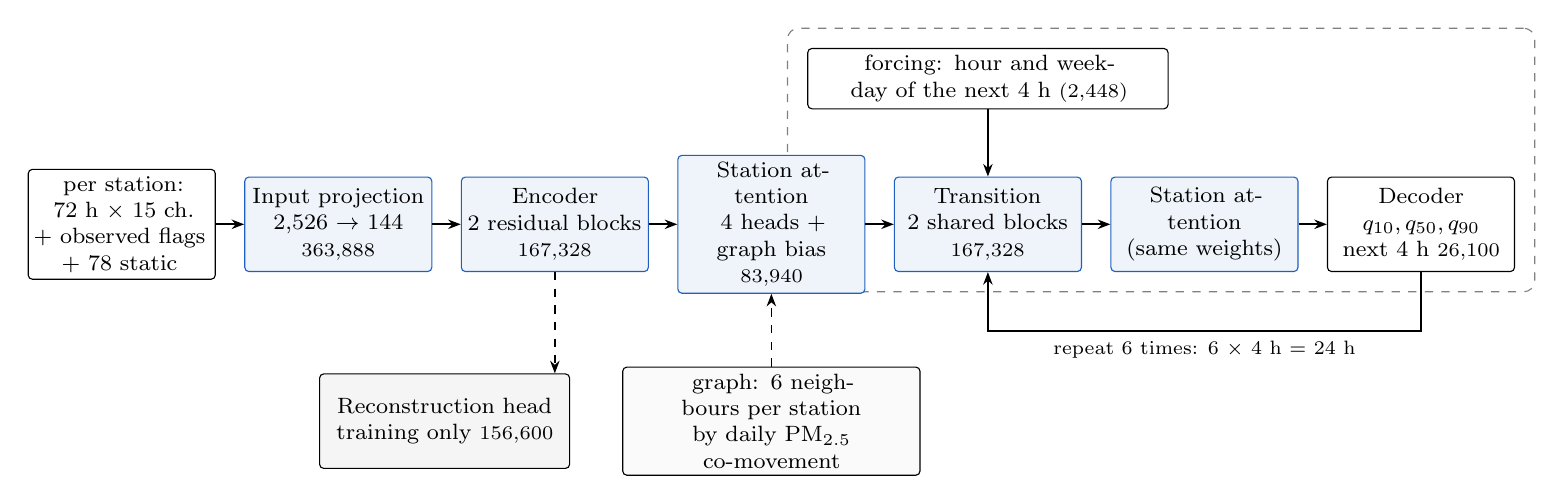
\begin{tikzpicture}[font=\footnotesize,
  box/.style={draw, rounded corners=1.5pt, align=center, inner sep=2.5pt, minimum height=12mm, text width=22mm, fill=white},
  hl/.style={box, draw=atlasblue, fill=atlasblue!7},
  arr/.style={-{Stealth[length=1.6mm]}, semithick}]
\node[box] (in) at (0,0) {per station:\\72 h $\times$ 15 ch.\\+ observed flags\\+ 78 static};
\node[hl] (inp) at (2.75,0) {Input projection\\2,526 $\to$ 144\\{\scriptsize 363,888}};
\node[hl] (enc) at (5.5,0) {Encoder\\2 residual blocks\\{\scriptsize 167,328}};
\node[hl] (att) at (8.25,0) {Station attention\\4 heads + graph bias\\{\scriptsize 83,940}};
\node[hl] (dyn) at (11.0,0) {Transition\\2 shared blocks\\{\scriptsize 167,328}};
\node[hl] (att2) at (13.75,0) {Station attention\\(same weights)};
\node[box] (dec) at (16.5,0) {Decoder\\$q_{10},q_{50},q_{90}$\\next 4 h {\scriptsize 26,100}};
\node[box, text width=44mm, minimum height=7mm] (f) at (11.0,1.85) {forcing: hour and weekday of the next 4 h {\scriptsize (2,448)}};
\node[box, fill=gray!8, text width=30mm] (rec) at (4.1,-2.5) {Reconstruction head\\training only {\scriptsize 156,600}};
\node[box, fill=gray!4, text width=36mm] (graph) at (8.25,-2.5) {graph: 6 neighbours per station\\by daily \pmtf{} co-movement};
\draw[arr] (in) -- (inp); \draw[arr] (inp) -- (enc); \draw[arr] (enc) -- (att); \draw[arr] (att) -- (dyn); \draw[arr] (dyn) -- (att2);
\draw[arr] (att2) -- (dec); \draw[arr] (f) -- (dyn); \draw[arr, dashed] (enc.south) -- (rec.north -| enc.south);
\draw[arr, dashed] (graph) -- (att);
\draw[arr] (dec.south) -- ++(0,-0.75) -| node[pos=0.25, below, font=\scriptsize] {repeat 6 times: 6 $\times$ 4 h = 24 h} (dyn.south);
\begin{scope}[on background layer]\node[draw=gray, dashed, rounded corners, fit=(dyn)(att2)(dec)(f), inner sep=2.5mm] {};\end{scope}
\end{tikzpicture}}
\caption{\textbf{Atlas} (967,632 parameters; per-part counts in small type, measured from the code). The encoder and the
first attention run once; transition, attention and decoder run six times, each step adding four hours of forcing.
The decoder starts at zero, so an untrained Atlas forecasts persistence; the quantiles are offsets from the last
observation that cannot cross. The forecasting path has 811,032 parameters.}
\label{fig:atlas}
\end{figure}

\paragraph{Atlas.} For each station of a network, Atlas reads 72 hours of 15 channels (four pollutant targets, four
other pollutants, six weather variables, solar radiation) with observed flags, and 78 static numbers (14 daily \pmtf{}
means, the value one week before each forecast hour, the log scale). Pollutant targets are divided by the station's own
mean over the past week, so one set of weights reads clean and polluted stations alike. The flattened input is
projected to a 144-wide state and passed through two residual blocks (LayerNorm, 144$\to$288, GELU, 288$\to$144).
Stations are mixed by four-head attention whose logits carry a bias learned from each pair's graph features (edge
weight, self-loop, edge); each station links to the six stations whose daily \pmtf{} co-moves most with its own, using
the training period for trained stations and only the validation period for never-trained ones. The 24 forecast hours
come from six latent steps of four hours: the state absorbs that block's calendar forcing, passes two shared residual
blocks, is mixed again across stations, and is decoded into three quantiles for every channel and hour
(Fig.~\ref{fig:atlas}). Training minimises pinball loss (weight 1.0 on \pmtf{}, 0.1 on other pollutants, 0.05 on
weather) plus 0.2 times the reconstruction of 0--40\% randomly hidden input cells, with AdamW. Table~\ref{tab:params}
gives the parameter budget: the station attention, the only part that lets one station use another, holds 8.7\%.

\begin{figure}[t]
\centering
\resizebox{\linewidth}{!}{%
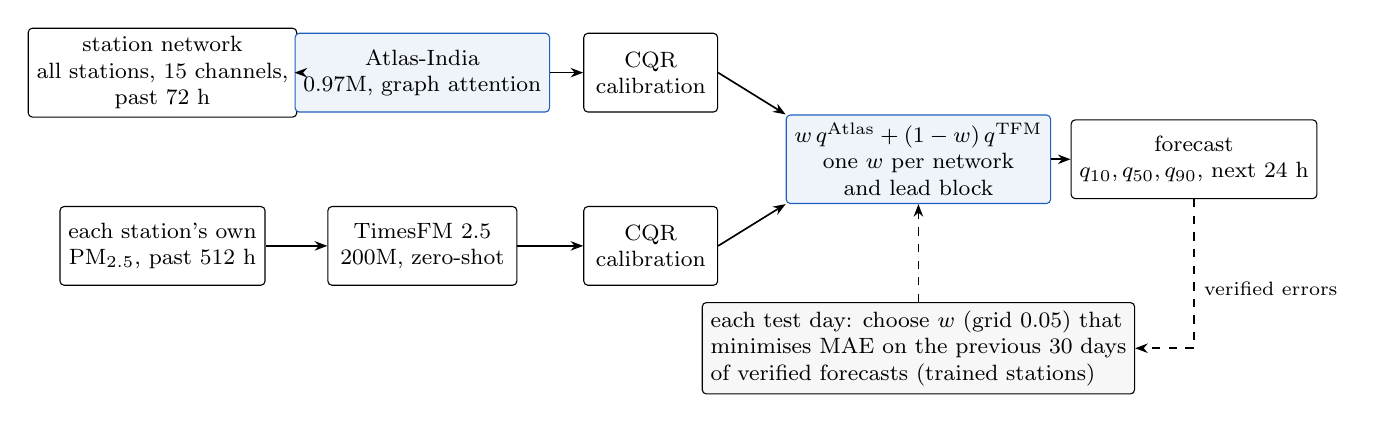
\begin{tikzpicture}[font=\footnotesize,
  box/.style={draw, rounded corners=1.5pt, align=center, inner sep=3pt, minimum height=10mm, minimum width=24mm, fill=white},
  hl/.style={box, draw=atlasblue, fill=atlasblue!7},
  arr/.style={-{Stealth[length=1.6mm]}, semithick}]
\node[box] (net) at (0,1.1) {station network\\all stations, 15 channels,\\past 72 h};
\node[box] (own) at (0,-1.1) {each station's own\\\pmtf{}, past 512 h};
\node[hl] (atlas) at (3.3,1.1) {Atlas-India\\0.97M, graph attention};
\node[box] (tfm) at (3.3,-1.1) {TimesFM 2.5\\200M, zero-shot};
\node[box, minimum width=17mm] (c1) at (6.2,1.1) {CQR\\calibration};
\node[box, minimum width=17mm] (c2) at (6.2,-1.1) {CQR\\calibration};
\node[hl, minimum width=33mm] (mix) at (9.6,0) {$w\,q^{\mathrm{Atlas}}+(1-w)\,q^{\mathrm{TFM}}$\\one $w$ per network\\and lead block};
\node[box, minimum width=20mm] (out) at (13.1,0) {forecast\\$q_{10},q_{50},q_{90}$, next 24 h};
\node[box, fill=gray!6, align=left, minimum width=46mm] (wsel) at (9.6,-2.4) {each test day: choose $w$ (grid 0.05) that\\minimises MAE on the previous 30 days\\of verified forecasts (trained stations)};
\draw[arr] (net) -- (atlas); \draw[arr] (own) -- (tfm); \draw[arr] (atlas) -- (c1); \draw[arr] (tfm) -- (c2);
\draw[arr] (c1.east) -- (mix.north west); \draw[arr] (c2.east) -- (mix.south west); \draw[arr] (mix) -- (out);
\draw[arr, dashed] (wsel) -- (mix);
\draw[arr, dashed] (out.south) |- node[pos=0.3, right, font=\scriptsize] {verified errors} (wsel.east);
\end{tikzpicture}}
\caption{\textbf{Atlas-F.} Two calibrated forecasts are averaged with a weight that is re-chosen every day from the
record of the previous 30 days only; never-trained stations reuse the weight fitted on trained stations.}
\label{fig:atlasf}
\end{figure}

\paragraph{Atlas-F.} Fig.~\ref{fig:atlasf} shows the fused system; \S\ref{sec:fusion} gives its rule and results.
The two members see different information: Atlas reads every station's 15 channels, TimesFM~2.5 reads one station's
\pmtf{} history. A weight learned from the recent record lets the system lean on whichever has been more accurate in
each network and at each lead time.

\begin{table}[t]
\caption{\textbf{Where Atlas's parameters sit} (counted from the code; totals match the trained checkpoints).}
\label{tab:params}
\centering\small
\begin{tabular}{llrr}
\toprule
Part & Role & Parameters & Share \\
\midrule
Input projection & 2,526 inputs per station $\to$ 144 & 363,888 & 37.6\% \\
Encoder & 2 residual blocks & 167,328 & 17.3\% \\
Transition & 2 shared residual blocks, run 6 times & 167,328 & 17.3\% \\
Reconstruction head & hidden-cell reconstruction (training only) & 156,600 & 16.2\% \\
Station attention & 4 heads, learned graph bias, shared across steps & 83,940 & 8.7\% \\
Decoder & 3 quantiles $\times$ 15 channels $\times$ 4 h & 26,100 & 2.7\% \\
Forcing embedding & hour and weekday of the next 4 h & 2,448 & 0.3\% \\
\midrule
Total & & 967,632 & \\
\bottomrule
\end{tabular}
\end{table}

% =================================================================================================================
\section{The confirmation test and the failure it found}
\label{sec:lono}

\begin{table}[t]
\caption{\textbf{Leave one network out.} Atlas pre-trained on the other 13 networks, adapted on the target's history as
in v1.3, scored on its all-India test windows (725 windows). MAE \trk{s} / \trk{u} in \pmu. Kaggle runs
atlas-lono-$\ast$ and atlas-lono-score.}
\label{tab:lono}
\centering\small
\resizebox{\linewidth}{!}{%
\begin{tabular}{lcccc l}
\toprule
Network & Adapted & Pre-trained only & TimesFM 2.5 & Atlas-India (all 14) & Verdict \\
\midrule
Uttar Pradesh & \textbf{21.45} / \textbf{23.14} & 21.76 / 23.29 & 22.78 / 24.32 & 20.89 / 22.46 & beats ($-5.8\%$, $p{=}2{\times}10^{-7}$ / $-4.8\%$, $p{=}3{\times}10^{-4}$) \\
Haryana & 24.93 / 22.85 & 25.31 / 23.17 & 25.72 / 23.20 & 24.32 / 22.31 & level ($-3.1\%$, $p{=}0.001$ / $-1.5\%$, $p{=}0.20$) \\
Maharashtra & 19.86 / 28.28 & 20.39 / 25.44 & 19.45 / \textbf{22.25} & 19.68 / 24.92 & loses ($+2.1\%$, $p{=}0.003$ / $+27.1\%$, $p{=}2{\times}10^{-19}$) \\
Karnataka & 8.97 / 9.68 & 9.26 / 9.44 & 8.98 / 9.43 & 8.87 / 9.20 & loses ($-0.1\%$, $p{=}0.96$ / $+2.7\%$, $p{=}0.03$) \\
\bottomrule
\end{tabular}}
\end{table}

The rule fixed before the runs required the v1.3 recipe, repeated with each of the four largest networks after Delhi
left out of pre-training, to beat TimesFM~2.5 on at least three and lose on none. It did not (Table~\ref{tab:lono}):
one win, one level, two losses; more seeds cannot change this because the Maharashtra loss is decisive. We had
predicted wins on Uttar Pradesh and Haryana and level on the other two.

Two findings follow. First, the gain is geographic: Delhi, Uttar Pradesh and Haryana share the Indo-Gangetic airshed
and its winter regime, Maharashtra and Karnataka do not. Second, the failure is at \emph{never-trained} stations of
spread-out networks. Adapting on Maharashtra's 22 trained stations raised its never-trained error from 25.44 to 28.28,
and even Atlas-India is 12\% behind TimesFM~2.5 there. Atlas mixes every station of a network by attention; only a
learned bias separates graph neighbours, whose links to never-trained stations come from 61 validation days. Where
cities are hundreds of kilometres apart, unrelated stations can outweigh related ones, a failure a univariate model
cannot have.

% =================================================================================================================
\section{Atlas-F: letting the record decide between Atlas and a foundation model}
\label{sec:fusion}

\paragraph{Method.} Atlas-F averages two calibrated forecasts, Atlas-India and TimesFM~2.5, with weight $w$ on Atlas:
\begin{equation}
\hat q^{F}_{t} = w_{t,b}\,\hat q^{\text{Atlas}}_{t} + (1-w_{t,b})\,\hat q^{\text{TimesFM}}_{t},
\end{equation}
with $w$ on a 0.05 grid, one weight per network and lead block $b$ (1--6, 7--12, 13--24 hours). At the start of each
test day $w$ is re-chosen to minimise MAE on the previous 30 days of forecasts whose 24 target hours were observed
before that day began (validation windows fill the first month), on trained stations only; never-trained stations reuse
it. Nothing from a forecast's future is used. The grid, the window and the blocks were fixed in the repository before
the run; TimesFM~2.5 is Apache-2.0 licensed, and no non-commercial model is a member.

\begin{table}[t]
\caption{\textbf{All-India league} (14 networks, 263 stations, 725 windows per network; third use of this test period).
Every entry calibrated on each network's validation windows. Kaggle run atlas-fusion-f (version 2).}
\label{tab:fusion}
\centering\small
\setlength{\tabcolsep}{4pt}\begin{tabular}{lcc l}
\toprule
Entry & \trk{s} MAE & \trk{u} MAE & Atlas-F against it (\trk{s} / \trk{u}) \\
\midrule
\textbf{Atlas-F} & \textbf{20.75} & \textbf{20.44} & -- \\
Atlas-India (v1.3, 3 seeds) & 20.99 & 20.86 & beats: $-1.16\%$ ($p{=}5{\times}10^{-14}$) / $-2.05\%$ ($p{=}6{\times}10^{-22}$) \\
TimesFM 2.5, zero-shot & 22.35 & 21.93 & beats: $-7.16\%$ ($p{=}10^{-37}$) / $-6.80\%$ ($p{=}10^{-28}$) \\
\bottomrule
\end{tabular}
\end{table}

\begin{figure}[t]
\centering
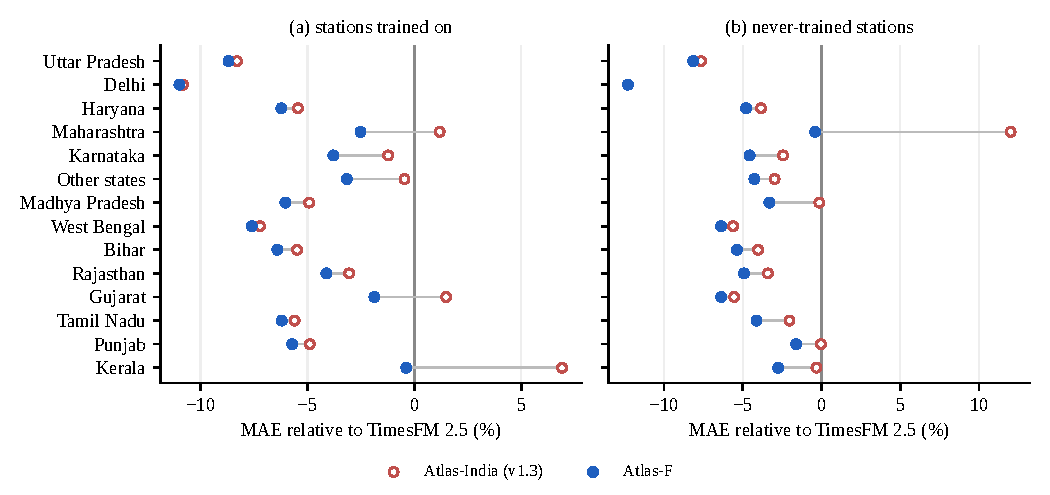
\includegraphics[width=\linewidth]{figures/fusion_networks.pdf}
\caption{\textbf{Network by network}, MAE relative to TimesFM~2.5. Atlas-India alone is worse than TimesFM~2.5 in
Maharashtra and Gujarat (trained stations), Kerala, and Maharashtra's never-trained stations ($+12\%$); Atlas-F is
better than TimesFM~2.5 in all 28 network-tracks.}
\label{fig:fusion}
\end{figure}

\paragraph{Results.} Atlas-F beats both of its members on both tracks (Table~\ref{tab:fusion}), and its MAE is below
TimesFM~2.5's in all 28 network-tracks (Fig.~\ref{fig:fusion}; smallest margins: Kerala trained stations 7.93 against
7.96, Maharashtra never-trained 22.16 against 22.25). The pre-registered dominance rule (beat both members pooled on
both tracks and lose to TimesFM~2.5 on no network-track) is therefore met; we had given it even odds. The weights
follow the confirmation test without being told it: the mean weight on Atlas is 0.86 in Delhi and 0.80 in Uttar Pradesh,
but 0.46 in Maharashtra, 0.42 in Gujarat and 0.23 in Kerala. Atlas-F repairs Atlas's worst cells: Maharashtra's
never-trained error falls from 24.92 to 22.16, and Kerala's trained-station error from 8.51 to 7.93.

\paragraph{A discarded run.} The first run of the scorer read Atlas-India forecasts made before a recorded input fix
(unscaled pressure or temperature at never-trained stations of Gujarat, Kerala and Punjab), which put Atlas-India's
never-trained error at 21.25 instead of 20.86. It was discarded; the scorer now re-forecasts with the fix and refuses
older files, and the reported run reproduces the recorded Atlas-India numbers before scoring Atlas-F.


% =================================================================================================================
\section{Comparison with India's operational forecasts}
\label{sec:india_ops}

\paragraph{What can be compared.} India's operational air-quality forecasts for Delhi are IITM's Air Quality Early
Warning System, built on WRF-Chem at 400~m~\citep{jena2021delhi400m}, and IMD's SILAM. Their portals show current
forecasts as maps and charts; neither publishes an archive of past station forecasts, so no paired significance test is
possible. An independent evaluation by CEEW~\citep{ceew2025} scraped both systems' Day-1 forecasts and scored them on
Delhi's spatially averaged hourly \pmtf{} for 1 October 2024 to 28 February 2025. We score Atlas on that quantity and
window.

\begin{figure}[t]
\centering
\resizebox{\linewidth}{!}{%
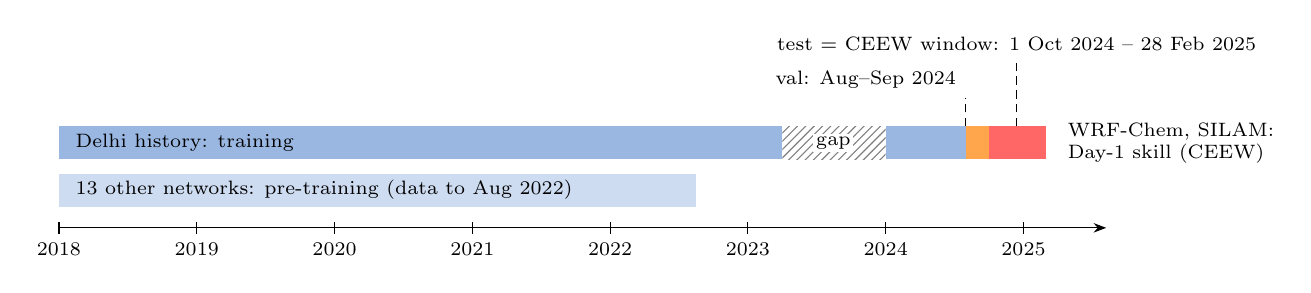
\begin{tikzpicture}[font=\footnotesize, x=1.75cm, y=0.6cm]
% x in years from 2018.0
\draw[-{Stealth[length=1.6mm]}] (0,0) -- (7.6,0);
\foreach \x/\l in {0/2018, 1/2019, 2/2020, 3/2021, 4/2022, 5/2023, 6/2024, 7/2025} {\draw (\x,0.12) -- (\x,-0.12) node[below] {\scriptsize \l};}
\fill[atlasblue!22] (0,0.45) rectangle (4.62,1.15); \node[font=\scriptsize, anchor=west] at (0.05,0.8) {13 other networks: pre-training (data to Aug 2022)};
\fill[atlasblue!45] (0,1.45) rectangle (5.25,2.15); \node[font=\scriptsize, anchor=west] at (0.05,1.8) {Delhi history: training};
\fill[pattern=north east lines, pattern color=gray] (5.25,1.45) rectangle (6.0,2.15); \node[font=\scriptsize, fill=white, inner sep=1pt] at (5.62,1.8) {gap};
\fill[atlasblue!45] (6.0,1.45) rectangle (6.58,2.15);
\fill[orange!70] (6.58,1.45) rectangle (6.75,2.15);
\fill[red!60] (6.75,1.45) rectangle (7.16,2.15);
\draw[densely dashed] (6.58,2.15) -- (6.58,2.75) node[above, font=\scriptsize, anchor=south east] {val: Aug--Sep 2024};
\draw[densely dashed] (6.95,2.15) -- (6.95,3.55) node[above, font=\scriptsize] {test = CEEW window: 1 Oct 2024 -- 28 Feb 2025};
\node[font=\scriptsize, anchor=west, align=left] at (7.25,1.8) {WRF-Chem, SILAM:\\Day-1 skill (CEEW)};
\end{tikzpicture}}
\caption{\textbf{Evaluation design of the comparison.} The Atlas scored here never saw data after 30 September 2024:
pre-trained on the 13 other networks (data to 2022), trained on Delhi's history to 31 July 2024 (with a gap from April
to December 2023 in the public record), validated on August--September 2024, and tested on the window CEEW used.}
\label{fig:i1design}
\end{figure}

\paragraph{Protocol.} The Atlas here is trained by the v1.3 recipe on nothing after 30 September 2024
(Fig.~\ref{fig:i1design}): pre-trained on the 13 other networks (the v1.3 checkpoints, seeds 320--322), then trained on
Delhi's history to 31 July 2024 and validated on August--September 2024, with the final stage chosen on validation.
Forecasts are issued at 00:00 IST every day for that day's 24 hours. The Delhi average at each hour is the mean over the
stations that reported \pmtf{} in that hour, for forecast and measurement alike; RMSE, MAE, mean bias, Pearson $r$ and
MAPE are computed on the hourly series, as in~\citep{ceew2025}. The rule fixed in advance: Atlas is said to have lower
error than a system only if both its MAE and RMSE are lower, and never to have beaten it significantly.

\begin{table}[t]
\caption{\textbf{Delhi, 1 October 2024 -- 28 February 2025}, spatially averaged hourly \pmtf{} (\pmu). Operational
systems: Day-1 forecasts as evaluated by CEEW~\citep{ceew2025}. Atlas: trained on nothing after 30 September 2024,
issued 00:00 IST, lead 1--24 h, three seeds, stage C chosen on validation; 151 days, 3{,}624 hours (CEEW: 3{,}512 stated). The two reference forecasts are computed on Atlas's series. Kaggle run atlas-i1-score. By number only.}
\label{tab:i1}
\centering\small
\setlength{\tabcolsep}{4pt}\begin{tabular}{lcccccc}
\toprule
Forecast & RMSE & MAE & Bias & $r$ & MAPE \% & Meas.\ mean \\
\midrule
\textbf{Atlas} (0.97M, sensors only) & \IoneRMSE & \IoneMAE & \IoneMBE & \IoneR & \IoneMAPE & \IoneObs \\
Same hour yesterday & 76.67 & 48.38 & $+0.33$ & 0.71 & 33 & 159 \\
Last observed value (23:00, held) & 83.32 & 56.27 & $+37.34$ & 0.74 & 50 & 159 \\
\midrule
IITM WRF-Chem 400 m (AQEWS), Day 1 & 92.53 & 58.75 & $-25.21$ & 0.61 & 35 & 175 \\
IMD SILAM, Day 1 & 107.95 & 71.68 & $-22.88$ & 0.47 & 45 & 177 \\
\bottomrule
\end{tabular}
\end{table}


\begin{figure}[t]
\centering
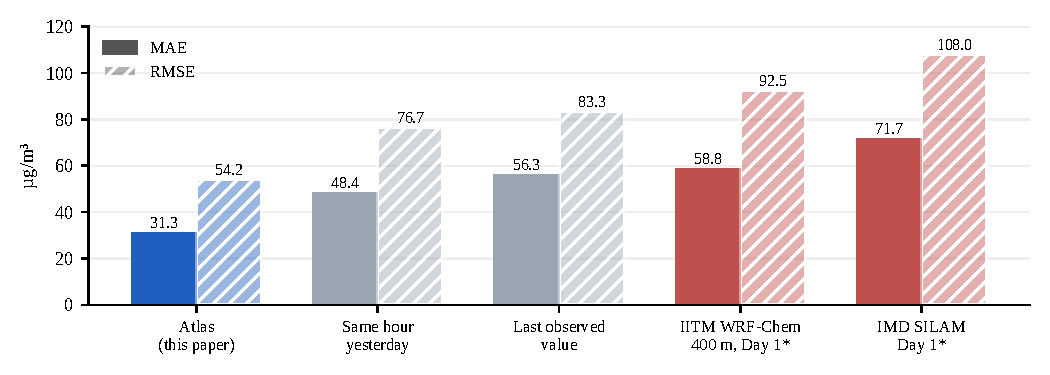
\includegraphics[width=\linewidth]{figures/i1_compare.pdf}
\caption{\textbf{Delhi, winter 2024--25: next-day error of Atlas against India's operational forecasts.} Delhi's
average hourly \pmtf{}, 1 October 2024 -- 28 February 2025. Atlas and the two persistence forecasts: our series
(3{,}624 hours, measured mean 159\,\pmu{}). *WRF-Chem and SILAM: values published by CEEW~\citep{ceew2025} on their
own observation set (3{,}512 hours, mean 175--177). By number only; no paired test is possible.}
\label{fig:i1}
\end{figure}

\paragraph{Result.} Atlas's error on Delhi's winter 2024--25 average is RMSE 54.24 and MAE 31.27\,\pmu{}, with a mean
bias of $-8.66$ and correlation 0.85 (Table~\ref{tab:i1}, Fig.~\ref{fig:i1}). Both its MAE and RMSE are below the published Day-1 values of
WRF-Chem (58.75, 92.53) and SILAM (71.68, 107.95), so by the rule fixed in advance Atlas has lower error \emph{by
number} than both. Every part of the advance prediction held: MAE in 25--40, RMSE in 35--60, both below the two systems,
and bias within $\pm15$. On the identical series, Atlas improves on same-hour-yesterday by 35\% (MAE) and 29\% (RMSE);
this is the like-for-like part of the result. Its bias is a third of the operational systems' (both under-predict by
about 23--25\,\pmu{}).

\paragraph{What the persistence rows show.} Not predicted, and important: even same-hour-yesterday (MAE 48.38, RMSE
76.67) is below both published values. Point error at 1--24\,h on measured station averages is where station-trained
forecasts are strongest and where a chemistry-transport model, which forecasts a city-wide field from emissions and
weather, is weakest; CEEW's ``Day 1'' may also be a longer lead. The observation sets also differ: our measured mean is
159\,\pmu{} against CEEW's 175--177. Scaled by each set's mean, Atlas's MAE is 20\% of the mean against WRF-Chem's 34\% and
SILAM's 40\%, so the ordering holds, but the size of the gap is uncertain. The result says Atlas is a much better next-day
point forecast of Delhi's measured average; it does not say Atlas could replace those systems.

\paragraph{Limits of this comparison.} (i) No paired test: the operational forecasts are not archived. (ii) CEEW does
not state its station set; our measured mean is shown beside theirs as a check. (iii) CEEW does not state the lead time
of ``Day 1''; if it is longer than Atlas's 1--24 hours, the comparison favours Atlas. (iv) The operational systems
forecast a city-wide field from emissions and meteorology and serve other purposes (attribution, emergency planning)
that a station model does not. (v) Winter 2023--24, CEEW's other season, cannot be scored: Delhi's public record has a
gap from April to December 2023.

% =================================================================================================================
\section{Experiments under way}
\label{sec:ongoing}

Both were pre-registered before their runs; no result is reported here.

\paragraph{Fixing the failure inside Atlas (v1.4).} Three candidates differ from Atlas-India in one respect each:
\emph{neighbour attention} (each station attends only to itself and its graph neighbours; 967,632 parameters), a
\emph{station gate} (a learned per-station gate on the attention update; 988,512), and both. The candidate with the
lowest validation MAE is adopted only if it is at least 1\% below Atlas-India's, and then tested once against
Atlas-India and TimesFM~2.5; it improves on v1.3 if it wins on at least one track and loses on neither.

\paragraph{The transfer threshold function.} On the four leave-one-out networks Atlas gets only the most recent
$B\in\{0,\tfrac12,1,2,4,8,16,\text{all}\}$ months of the target's data, trained from scratch or from the 13-network
checkpoint. We fit the scratch law $r=c_X+a\,n^{-\alpha}$ (relative error against TimesFM~2.5, $n$ local windows) and
the data transferred by pre-training, $D_T(n)=n_{\mathrm{eq}}-n$~\citep{hernandez2021scaling}. The rule: pre-training
lowers the data threshold if it reaches TimesFM~2.5's level with fewer months than scratch on at least three of four
networks.

% =================================================================================================================
\section{Limitations and conclusion}
\label{sec:conclusion}

\paragraph{Limitations.} Everything here is \pmtf{} at Indian stations, 24 hours ahead. The all-India test period has
now been used three times; Atlas-F's free choices were fixed before its run, but a fresh test period would make the
claim cleaner. Atlas-F depends on a 200M-parameter member, so it is not a small model; its value is that a small,
domain-trained model and a general one, weighed by their recent record, beat both. The comparison with India's
operational forecasts is by number, on a different station set and possibly a different lead time. The station-graph
failure is repaired by fusion, not yet inside Atlas.

\paragraph{Conclusion.} The first paper's claim survived its confirmation test only in the Indo-Gangetic plain. The test
located the failure (never-trained stations in spread-out networks), and a fused system whose weights are learned from
the trailing month repairs it: Atlas-F beats both Atlas and TimesFM~2.5 across India and TimesFM~2.5 in every network.
Set against India's operational forecasts on the quantity an independent evaluation used, an Atlas trained
on nothing after September 2024 has lower next-day error than IITM's WRF-Chem and IMD's SILAM by number (MAE 31.3 against
58.8 and 71.7\,\pmu{}), with the comparison's limits, above all that persistence is also below their published errors,
stated beside it. The priority now is a fix inside Atlas for spread-out networks (\S\ref{sec:ongoing}) and a paired
comparison, which needs the operational forecasts to be archived.

\ifpreprint
\paragraph{Code and data.} Code, every rule and prediction in the order written, and the notebooks that produced every
number: \url{https://github.com/paradoxailab/paradox-world-model} (branch \texttt{atlas-v0.1}). No data, weights or
keys are stored; all data are public.
\else
\paragraph{Code and data.} Code, the time-stamped rules and the notebooks are in a public repository whose link is
withheld for review.
\fi

\bibliographystyle{plainnat}
\bibliography{refs}

\end{document}
